\chapter{Numerical Framework}
\section{Introduction}
The collision of liquid jets has been studied in three-dimensional finite volume framework. Open source freeware, transient, multi-fluid, Navier-Stokes solver Gerris is used for the current study. Developed by \cite{Popinet2003,popinet2009}, Gerris has provided a stable and accurate platform for surface tension inclusive flows. It has been successful used frequently by researchers, such as \cite{chen2013high,kumar2016physical,kumar2017bending,kumar2017air}, to delve into similar problems in interfacial flows involving liquid sheets, jet and thin features like ligaments and films to capture intricate flow details and investigate the process. In this chapter, the detailed numerical framework adopted by Gerris is given. First, the governing equations and the corresponding discretization schemes are discussed followed by an illustration of the adaptive mesh refinement and grid independence study. At the end, a brief description about the work to validate the numerical model is presented.   
\section{Governing equations}
Conventional mass and momentum conservation equations for incompressible flow have been solved in presence of the surface tension and gravitational force. Equation~\ref{Equation::massConservation} contains the mass conservation equation for incompressible flow, which simply states that the velocity field ($V_i = V_1\hat{i} + V_2\hat{j} + V_3\hat{k}$) must be divergence free. 
\begin{equation}\label{Equation::massConservation}
\frac{\partial V_i}{\partial x_i} = 0
\end{equation}
The momentum equation for the incompressible Newtonian fluids that is solved for all the spatial coordinates can be summarized as given in equation~\ref{Equation::NS}. In the equation, the forces applied on the control volume chosen consist of the pressure in form of its gradient $\left(\frac{\partial P}{\partial x_i}\right)$, the volume specific body force due to gravitation $\left(\rho g_i\right)$, the surface forces due to shear stress ($2\mu D_{i,k}$, where $\mu$ represents the coefficient of dynamic viscosity and $D_{i,k} is the deformation tensor$) and the interface specific surface tension force ($\sigma \kappa$, where $\sigma$ is the surface tension coefficient and $\kappa$ denotes the curvature of the interface). 
\begin{equation}\label{Equation::NS}
\rho\left(\frac{\partial V_i}{\partial t} + V_k\frac{\partial V_i}{\partial x_k}\right) = -\frac{\partial P}{\partial x_i} + \frac{\partial(2\mu D_{i,k})}{\partial x_k} + \sigma\kappa\delta_sm_i + \rho g_i
\end{equation}
Moreover, the surface tension term is multiplied with the Dirac distribution function ($\delta_s$) to ensure that the force due to surface tension acts only at the interface having a normal vector $m_i$. Further, the deformation tensor $D_{i,k}$ is defined using the symmetric part of the velocity field gradient as given in equation~\ref{Equation::deformation}.
\begin{equation}\label{Equation::deformation}
D_{i,k} = \frac{1}{2}\left(\frac{\partial V_i}{\partial x_k} + \frac{\partial V_k}{\partial x_i}\right)
\end{equation}
The equation~\ref{Equation::NS} implicitly takes care of the mechanical energy. Moreover, the temperature variations are too small to affect the phenomenon being investigated and therefore, no thermal energy equation is considered. The interface tracking is done using the Volume Of Fluid (VOF), a front capturing approach involving volume fraction of liquid, defined as $\Psi(x_i, t)$, at the spatial and temporal instance of $x_i$ and $t$ respectively. The density and viscosity for the study can be described using equation~\ref{Equation::general} in terms of a generic property $A$.
\begin{equation} \label{Equation::general}
A (\Psi) = \Psi A_1 + (1-\Psi)A_2 \: \: \:  \forall  \: A \in \{\rho, \mu\}
\end{equation}
The VOF approach is implemented in a two-step process of interface reconstruction (based on the values of $\Psi$ and piecewise linear interface construction scheme, PLIC) along with geometric flux computation and interface advection, shown in equation~\ref{Equation::vof}.
\begin{equation} \label{Equation::vof}
\frac{\partial \Psi}{\partial t} + \frac{\partial(\Psi V_i)}{\partial X_i} = 0
\end{equation}
Gerris uses second-order accurate time discretization of momentum and continuity equations with time splitting algorithm as proposed by \cite{Chorin1968}, whereby an unconditionally stable corrector predictor time marching approach is adopted. A multigrid solver is used for the solution of the resulting pressure-velocity coupled Laplace equation. The advection term of the momentum equation $\left(V_k\frac{\partial V_i}{\partial X_k}\right)$ is estimated using the Bell-Colella-Glaz second-order unsplit upwind scheme \citep{bell1989second}, which requires the restriction to be set up on the time step. Following \cite{popinet2009}, time step has been determined to satisfy Courant-Friedrich-Lewy (CFL) stability criteria of less than unity. The details of solution procedure can be found in the works of \cite{Popinet2003,popinet2009}. In the next section, we have looked at the different process parameters which are relevant to this study followed by a grid independence study of the results.\\
\section{Process parameters and mesh sensitivity analysis}\label{sec::process}
The computational domain is also illustrated in figure~\ref{Figure::schematic}(a) with parabolic inflow (equation~\ref{Equation::parabolic} as suggested by \cite{choo2007effect}) of jets (diameter, $d_j$ and impingement angle, $2\alpha$) and boundary outflow elsewhere. In equation~\ref{Equation::parabolic}, $u_n$ is the inlet velocity, $u_j$ is the average velocity, $r$ is the radial location in the jet from its centerline and $d_j$ is the jet diameter.
\begin{equation}\label{Equation::parabolic}
\frac{u_n}{u_j} = 2\left(1 - \left(\frac{2r}{d_j}\right)^2\right) 
\end{equation}
Following equations~\ref{Equation::massConservation} to~\ref{Equation::parabolic}, one can easily see that the different features of the liquid sheets can be represented in terms of the kinematic and dynamic properties, such as jet velocity ($u_j$), its diameter ($d_j$), angle of impingement (2$\alpha$), acceleration due to gravity ($g$) and other physical properties such as the density of the fluid ($\rho$), its viscosity ($\mu$) and the coefficient of surface tension ($\sigma$) at the fluid-air interface. On performing non-dimensional analysis, it can be observed that Froude number $\left(Fr = \frac{u_j}{\sqrt{gd_j}}\right)$, Bond number $\left(Bo = \frac{\rho gd_j^2}{\sigma}\right)$ and ratio between Reynolds number and jet Froude number $\left(Re/Fr = \frac{\rho\sqrt{gd_j^3}}{\mu}\right)$ govern the shape and sizes of different links in the fluid chain structure. \\
\begin{figure}
	\centering
	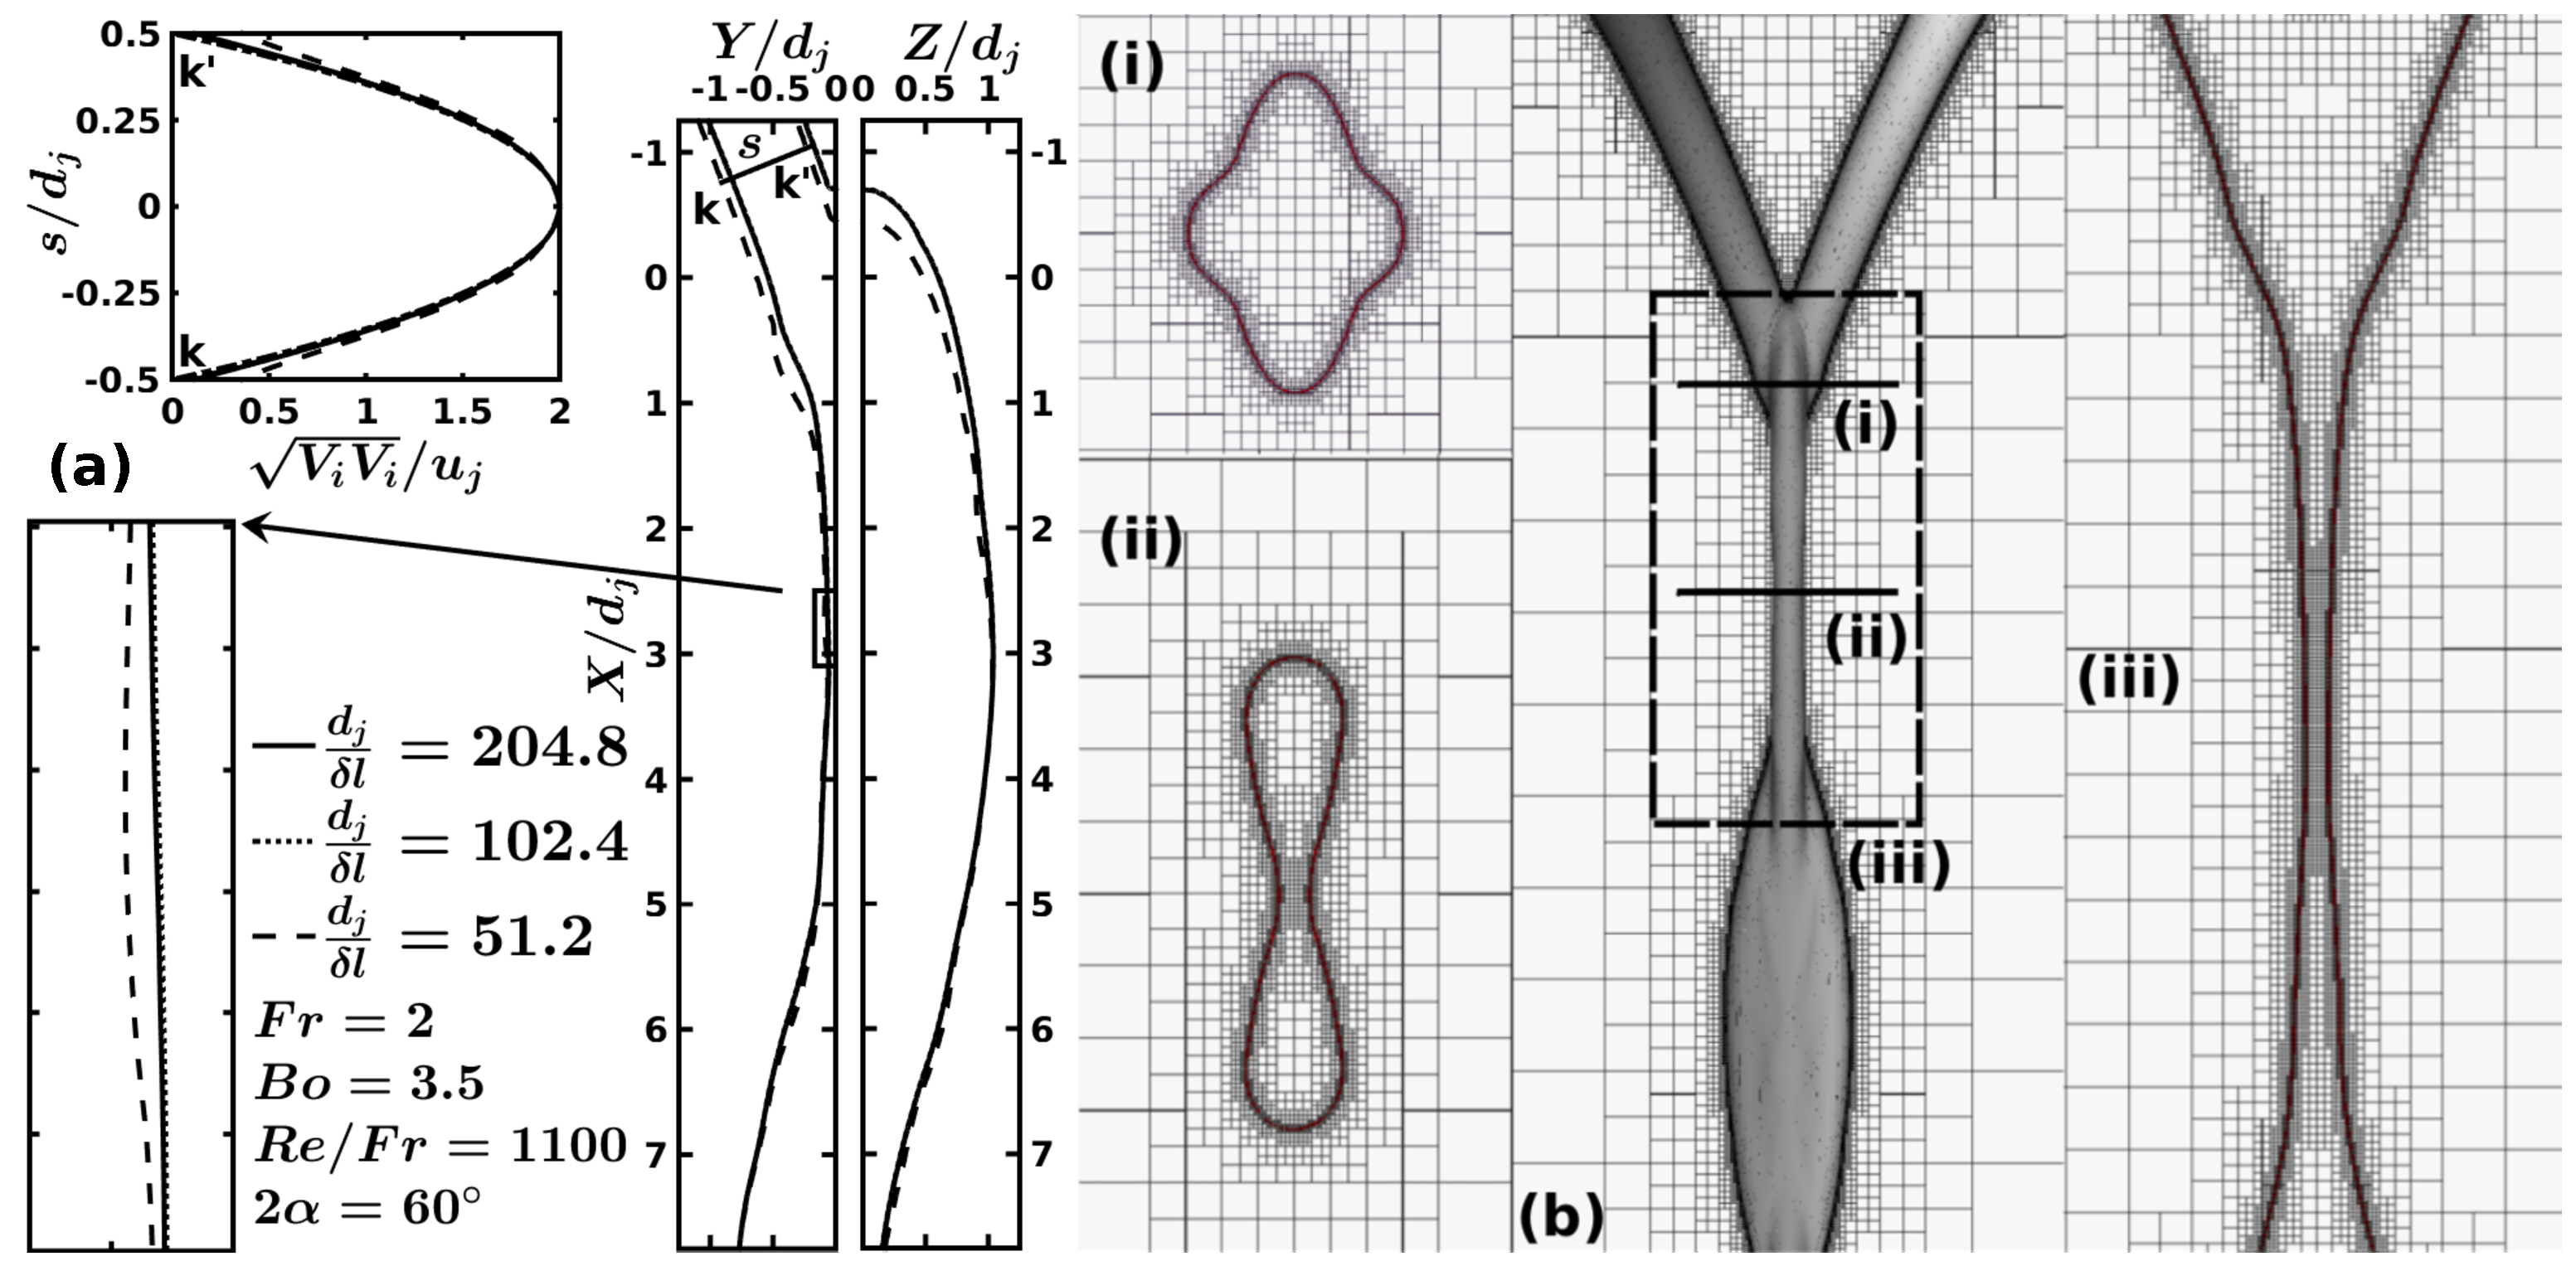
\includegraphics[width=\textwidth]{chapters/Figure2}
	\caption{(a) Mesh sensitivity analysis for a representative chain structure with the outer periphery and velocity profile near the inlet and (b) representation of the Adaptive Mesh Refinement (AMR) technique at critical locations.}
	\label{Figure::gisetal}
\end{figure}
The spatial discretization of the domain is undertaken using an octree-based structured hierarchical grid system, locally refined near the interface. It is necessary to capture the smallest features of the flow, in this case, the thickness of the liquid sheet. The multi-level grid structure adapts itself according to the gradient of the tracer $\Phi$, which implies that the structured octree mesh is finest at the interface between the two fluids. \cite{hasson1964thickness,choo2001parametric} have shown that the thickness of the liquid sheet can be given by the equation~\ref{Equation::thickness}. This expression has been found to describe the thickness of the liquid sheet within experimental precision by several independent researchers \citep{poulikakos1998thickness,choo2001parametric,ekimova2015liquid}.
\begin{equation}\label{Equation::thickness}
\frac{hr}{d_j^2} = \frac{1}{4}\frac{\sin^2\alpha}{(1-\cos\theta\cos\alpha)^2}
\end{equation} 
Here, $r$ is the radial direction originating from the collision point of the jets and $h$ is the measurement of the thickness of the film produced. Even though minima of equation~\ref{Equation::thickness} occurs at $\theta \to \pi$, it must be noted that the decrement in thickness is more prominent because of the increase in radial distance downstream of the first collision point $\left(h \propto \frac{1}{r}\right)$. Further, it can also be shown that the thickness of liquid sheet follows $\frac{hr}{d_j^2} \sim 1$, for $2\alpha \in \{0,\pi/2\}$. We maintained $\frac{d_j}{\delta l} \sim 10\frac{r_{max}}{d_j}$ to choose minimum cell size $\left(\delta l\right)$ and perform Grid Independence Study (GIS). The factor of 10 is included to have at least 10 grid points \citep{ling2015multiscale} across the smallest length scale for the structure to avoid breakage of sheet \citep{chen2013high}. To obtain good liquid film resolution, $\delta l$ is varied to match the above-mentioned criteria. In one representative simulation, we show the effect of variation of $\delta l$, in figure~\ref{Figure::gisetal} (a), on the sheet profile and velocity pattern of the jet. It can be observed that at $\frac{d_j}{\delta l}$ = 102.4, well resolved film is obtained with acceptable computational cost ($\sim 50\%$ less than $\frac{d_j}{\delta l}$ = 204.8). The results from this mesh sensitivity result have been summarized in table~\ref{Table::gis}. Mesh structure around different critical parts of the chain is shown in figure~\ref{Figure::gisetal}(b) which establishes sufficiency of grid points even inside smallest thickness of the film. In the next section, the validation of the employed numerical method is demonstrated.
\begin{table}[b]
\centering
\caption{Performance data of the processors used for simulations to determine the refinement level in the Grid Independence Study. The simulations are done using four Intel Core i7-6500U CPU having clock speed of 2.5GHz each and 8 GB RAM.}
\label{Table::gis}
\begin{tabular}{@{}cc@{}}
\toprule
$\left(\frac{d_j}{\delta l}\right)_{max}$ &\begin{tabular}[c]{@{}c@{}}$\left(\frac{t_{CPU}}{t_{actual}}\right)$\\ (days/s)\end{tabular} \\ \midrule
51.2                   & $\sim$ 20 \\
102.4                  & $\sim$ 28 \\
204.8                  & $\sim$ 60 \\ \bottomrule
\end{tabular}
\end{table} 
\section{Validation of the numerical model}
To check the accuracy of the developed mesh structure, results from simulations are compared with experimental observations obtained by \cite{bush2004collision}. Figure~\ref{Figure::validation} presents a description of the results in this test. The one-to-one correspondence between the experimental sheet profile \citep{bush2004collision} and the numerical results is reported in figure~\ref{Figure::validation}(a). Making use of the fact that their experiments led to supercritical (greater than capillary wave speed) sheet speeds, \cite{bush2004collision} were able to construct the variation of liquid volume flux $\left(Q(\theta) = \frac{dQ}{d\theta} = uhr\right)$ inside the sheet by scanning across the sheet and collecting liquid through a fine opening. In order to get quantitative validation, the variation of liquid volume flux ($Q(\theta)$) inside the sheet is also plotted in figure~\ref{Figure::validation}(b) along with \cite{bush2004collision}. Matching between present numerical simulations and pioneering experimental result by \cite{bush2004collision} provides confidence for the numerical understanding of the phenomenon, in our work. In the next chapter, results of the numerical simulation using the presented model to study the collision of liquid jets are summarized.
\begin{figure}
	\centering
	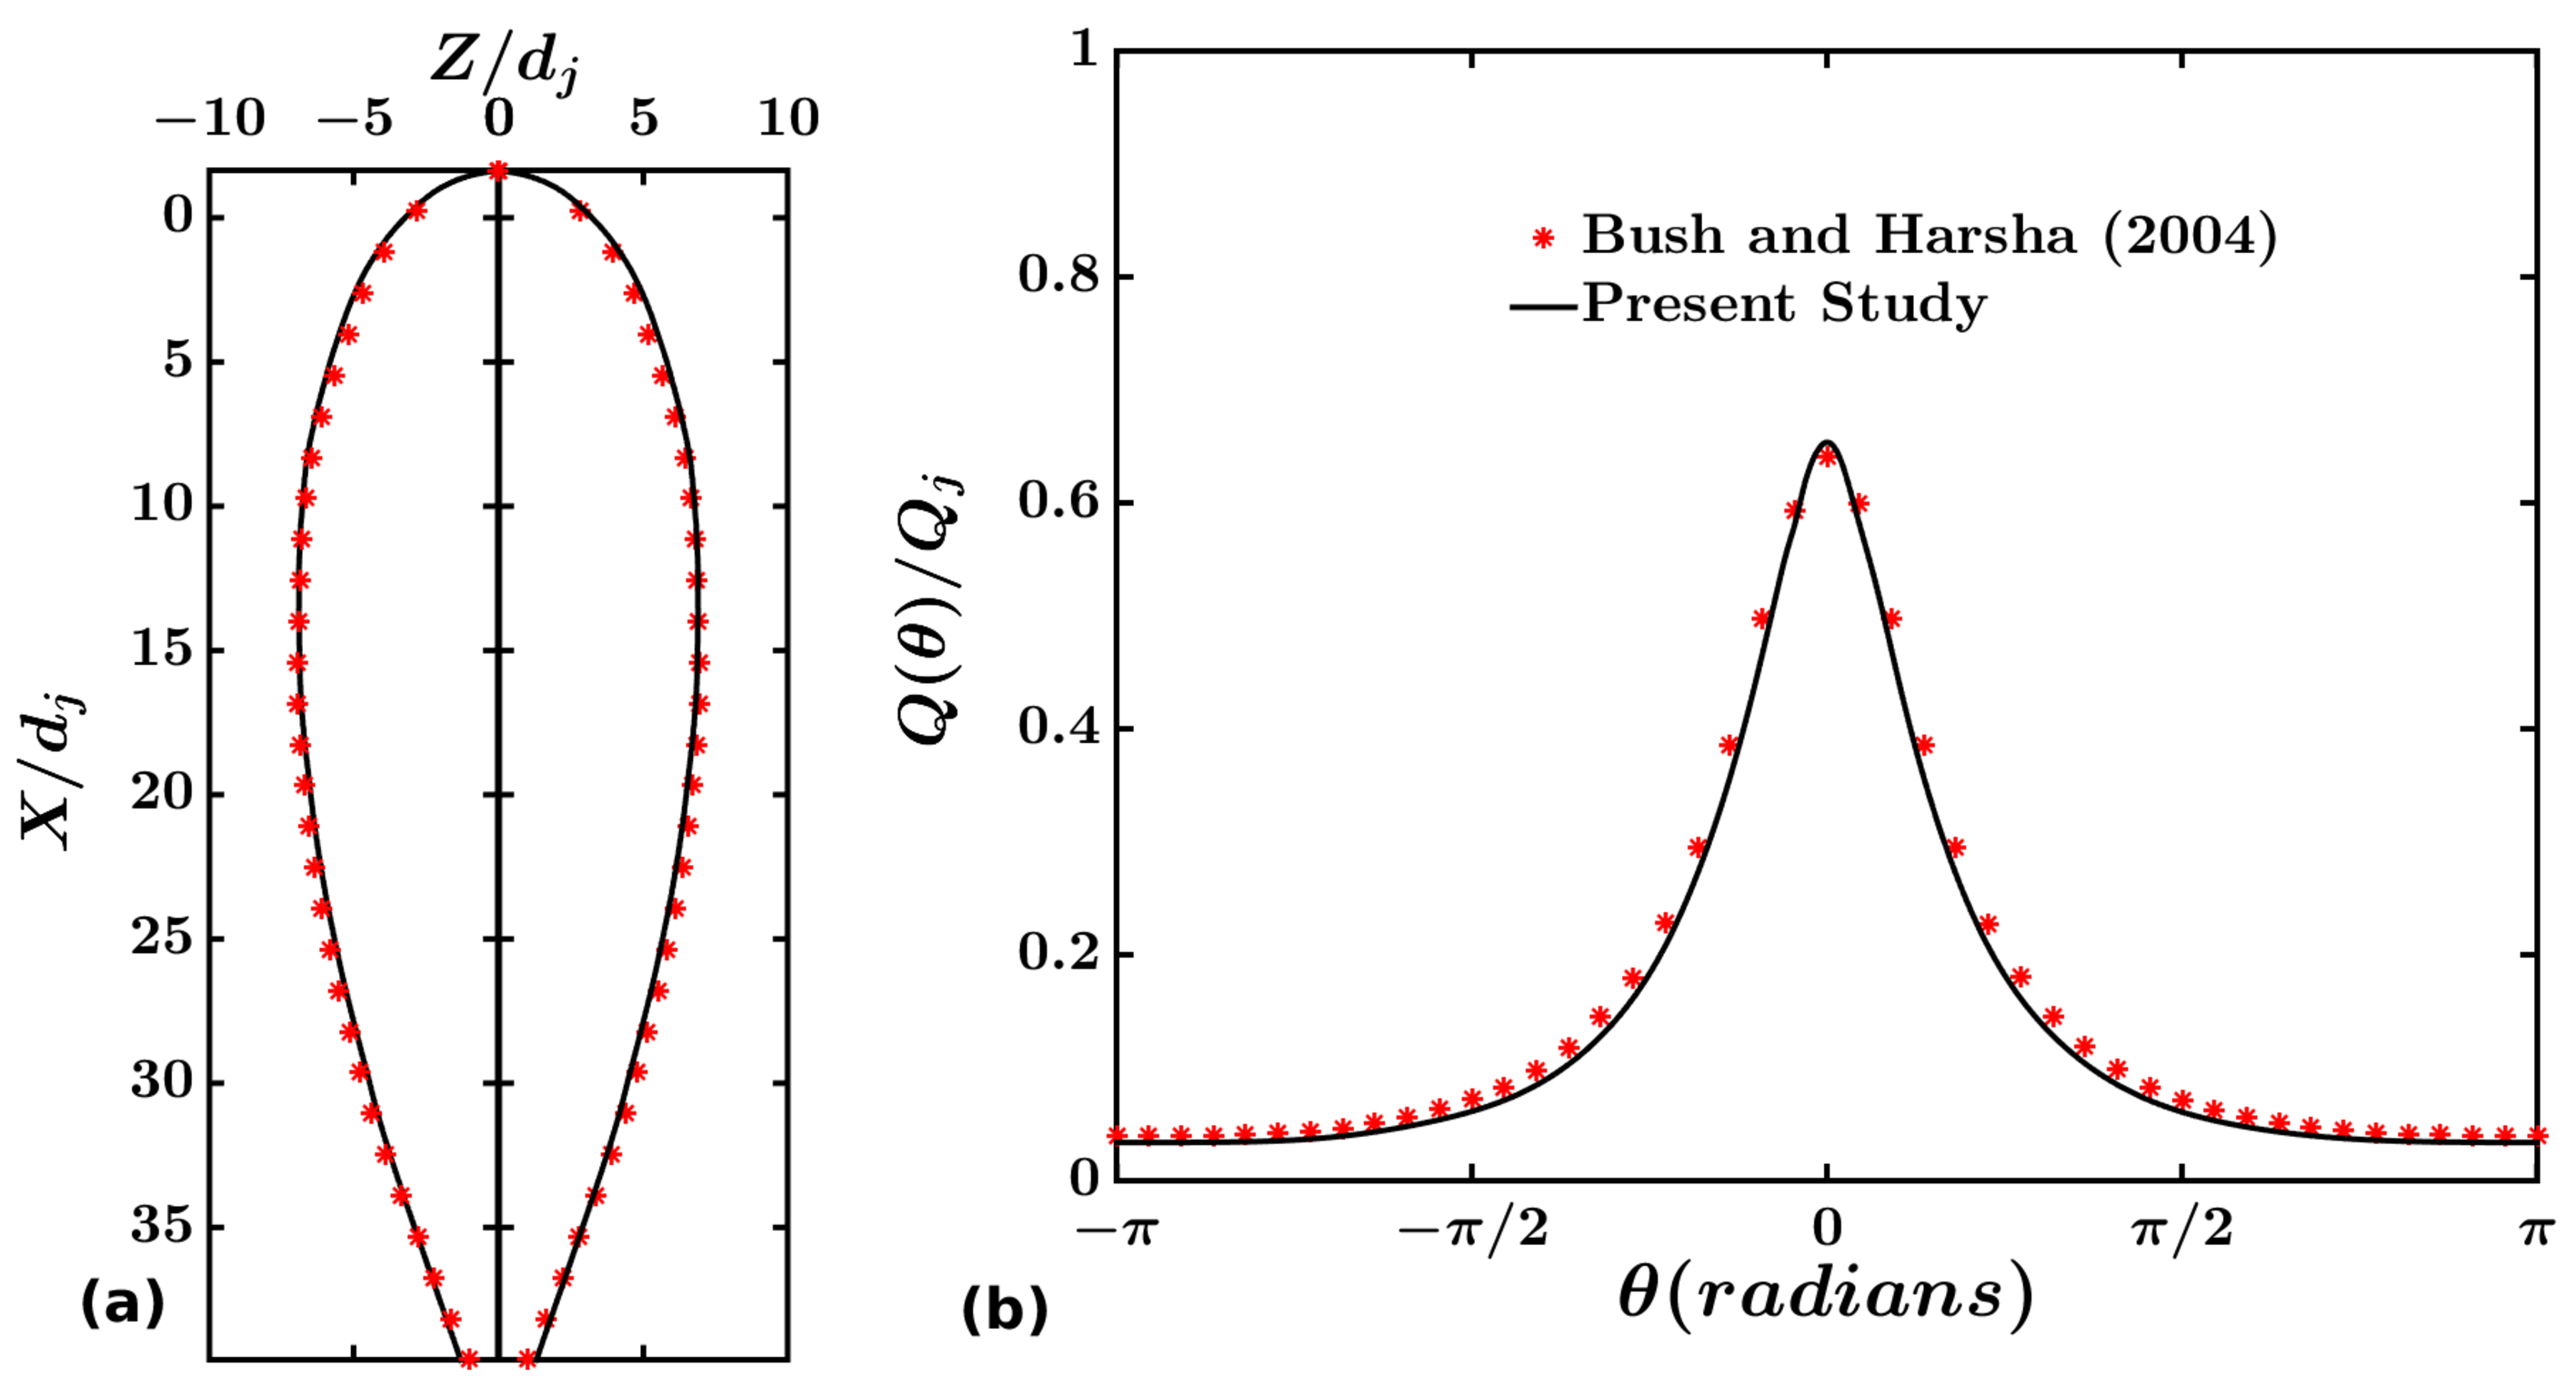
\includegraphics[width=\linewidth]{chapters/Figure3}
	\caption{Illustration of the validation of numerical model undertaken by comparison of (a) numerical interface and (b) liquid flux variation with the azimuthal angle, $\theta$. The numerically obtained results are superimposed with the respective experimental values obtained by \cite{bush2004collision}.}
	\label{Figure::validation}
\end{figure}